\section{Measurements}
\label{sec:measurements}

\subsection{Preparations and calibration of the setup}
\label{sub:preparations_and_calibration_of_the_setup}
First we measured the signal from the detector and Photomultiplier. We noticed
that the peaks of shape were at irregular points in time. We exchanged the left for the right side
of the photomultiplier, but did not observe a crucial dependence. Also rotating the sample did not
change the result significantly. Now we removed the oscilloscope and appended the Multichannelanalyzer,
in order to measure the energy spectrum. 
\subsubsection{Measuring the full energy spectrum}
\label{ssub:Measuring the full energy spectrum}
Our first configuration of the MA1 was the following:
\begin{tabular}{l|l}
    x & x
\end{tabular}

\begin{figure}
    \begin{subfigure}[b]{\picwidth}
        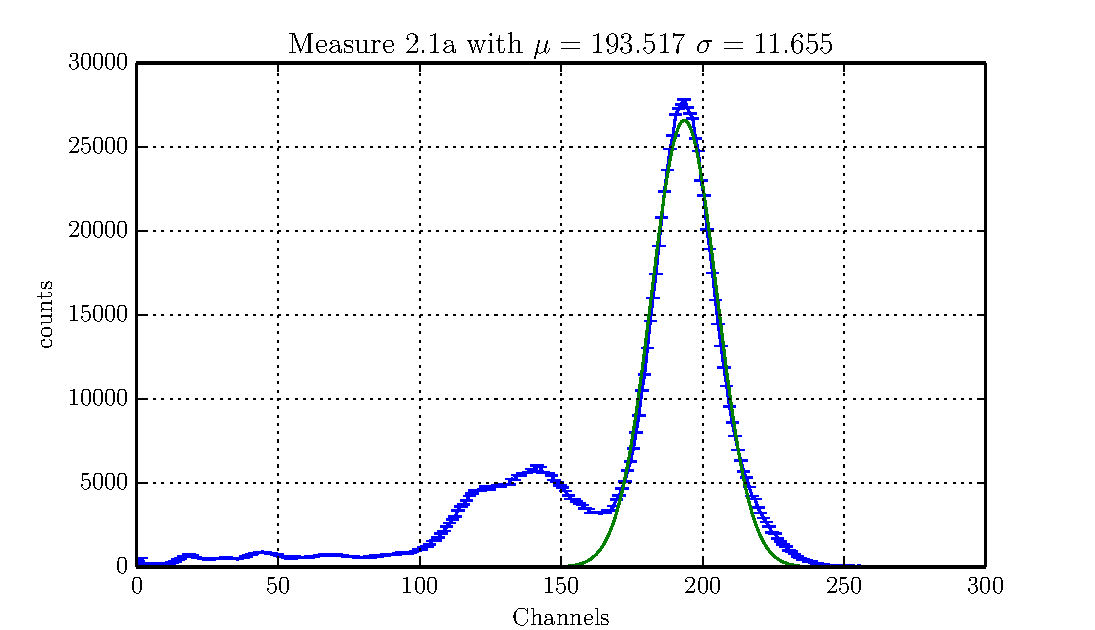
\includegraphics[width=\textwidth]{analysis/figures/plot2_1a}
        \caption{}
    \end{subfigure}\qquad
    \begin{subfigure}[b]{\picwidth}
        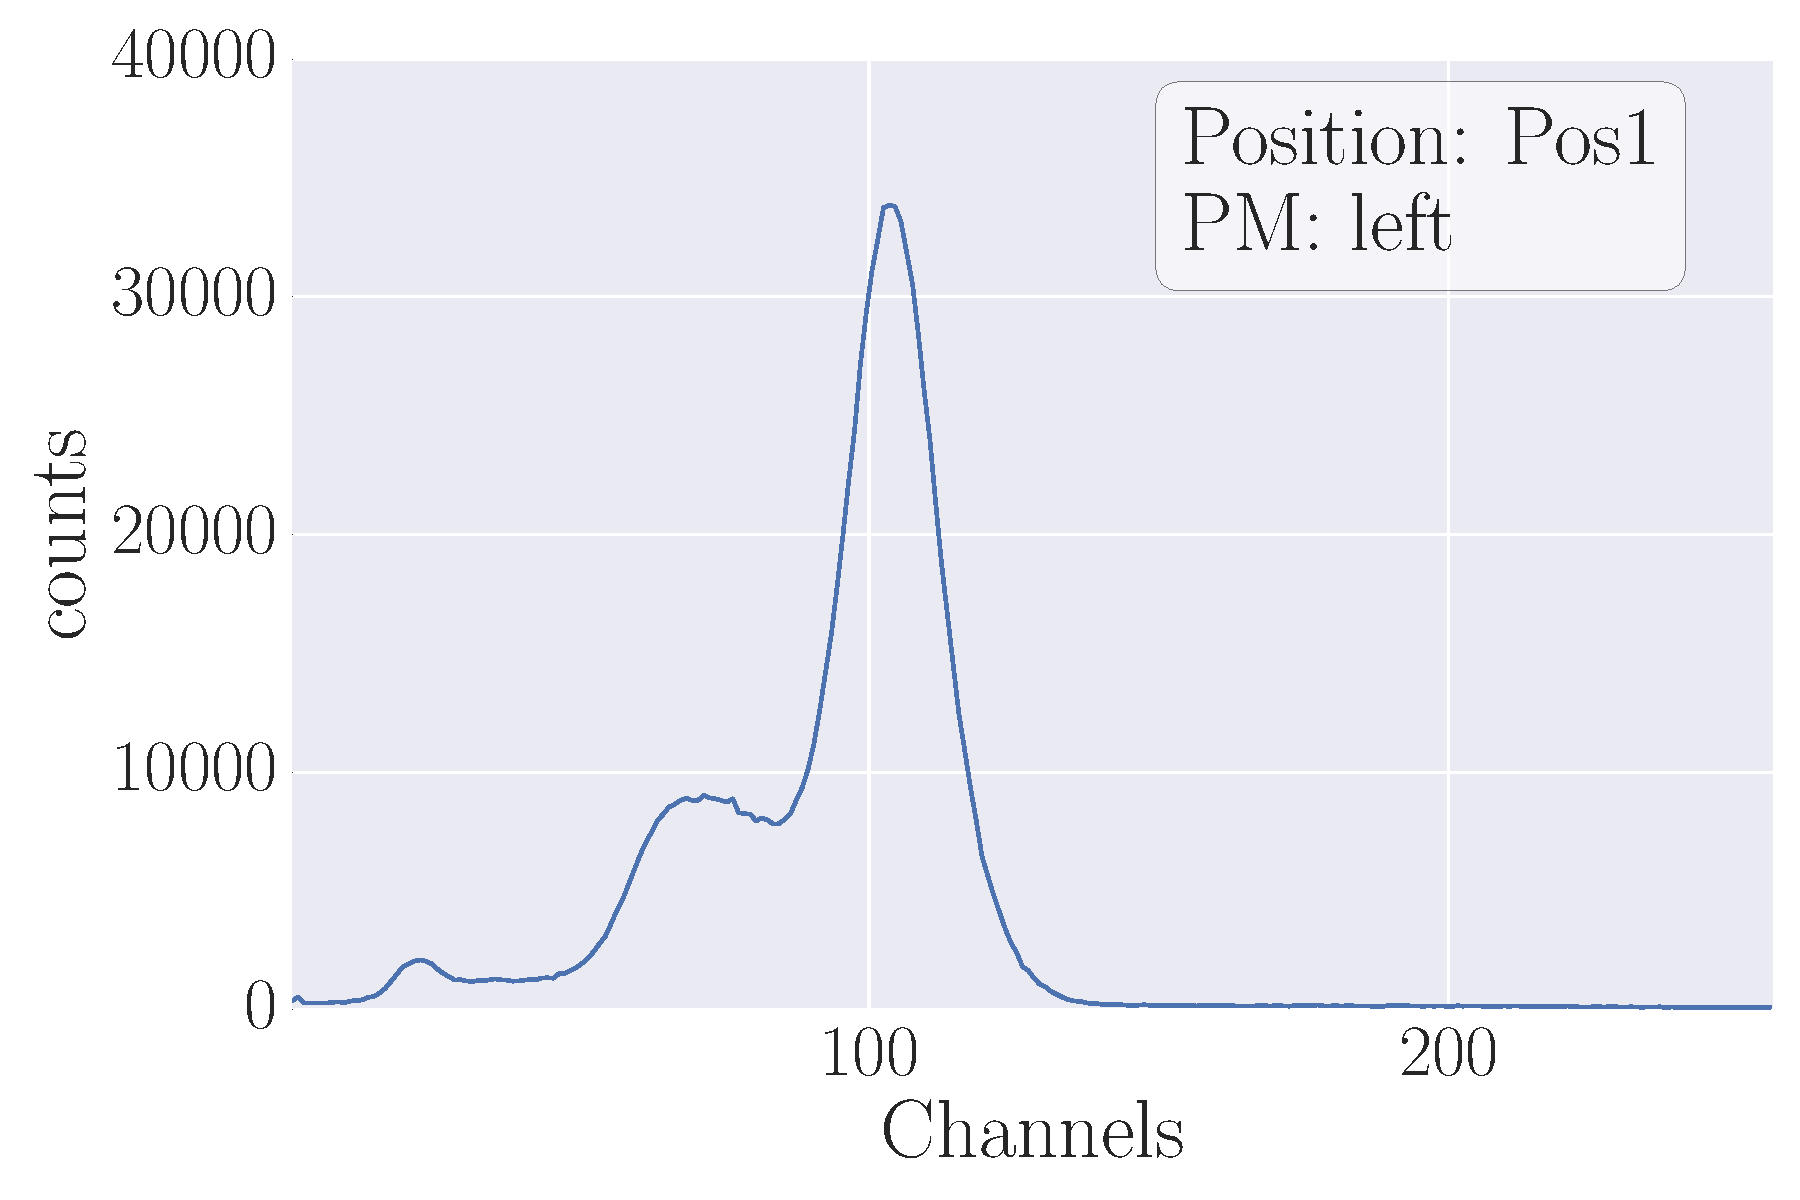
\includegraphics[width=\textwidth]{analysis/figures/plot2_1b}
        \caption{}
    \end{subfigure}
    \begin{subfigure}[b]{\picwidth}
        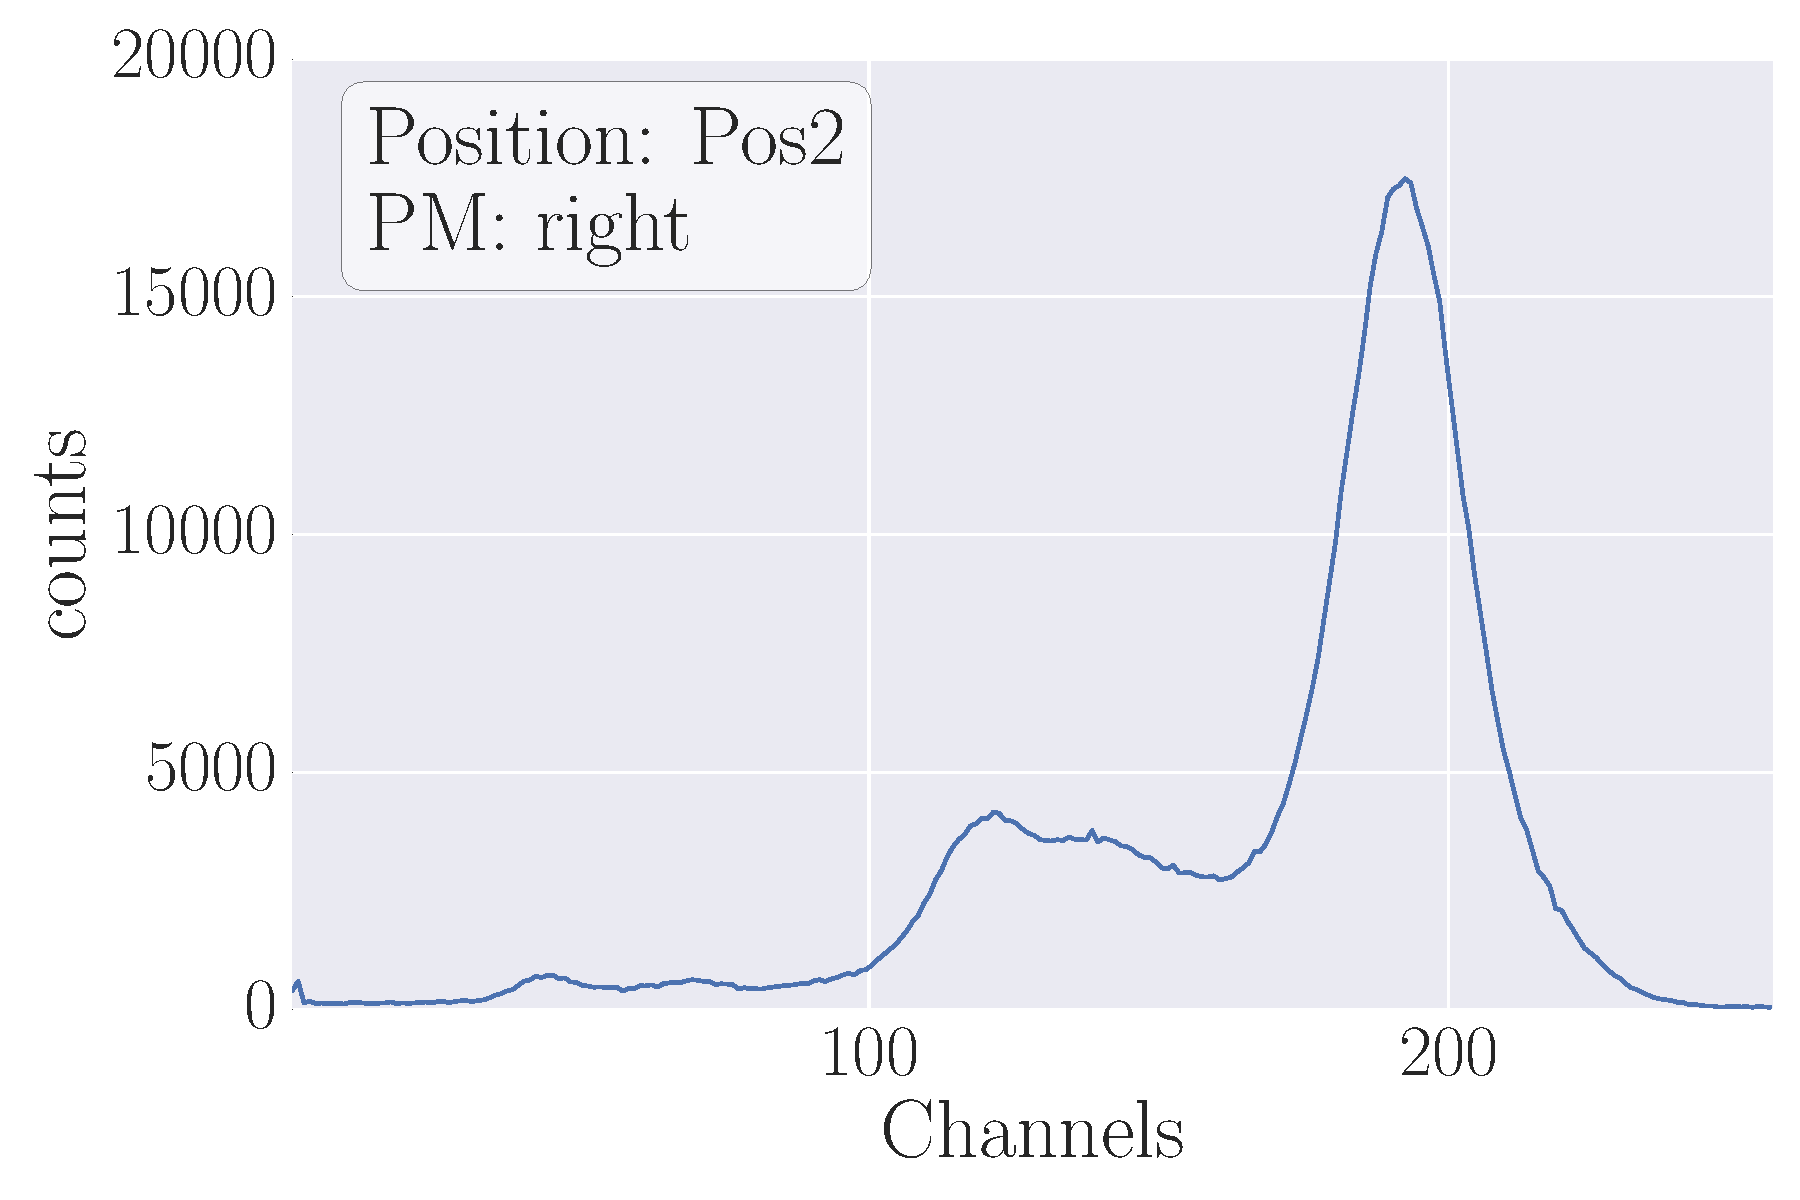
\includegraphics[width=\textwidth]{analysis/figures/plot2_1c}
        \caption{}
    \end{subfigure}
    \begin{subfigure}[b]{\picwidth}
        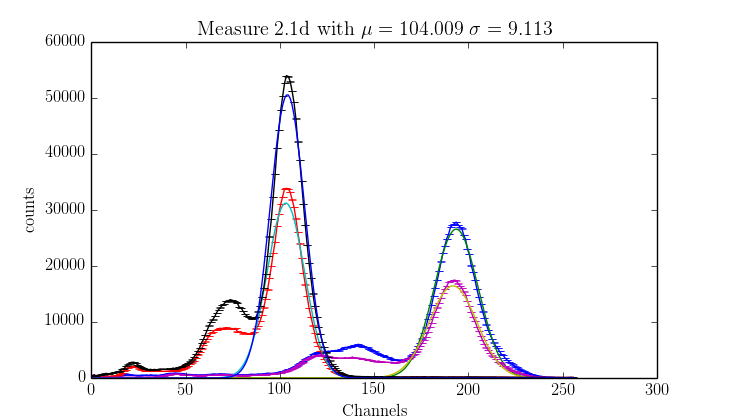
\includegraphics[width=\textwidth]{analysis/figures/plot2_1d}
        \caption{}
    \end{subfigure}
    \begin{subfigure}[b]{\picwidth}
        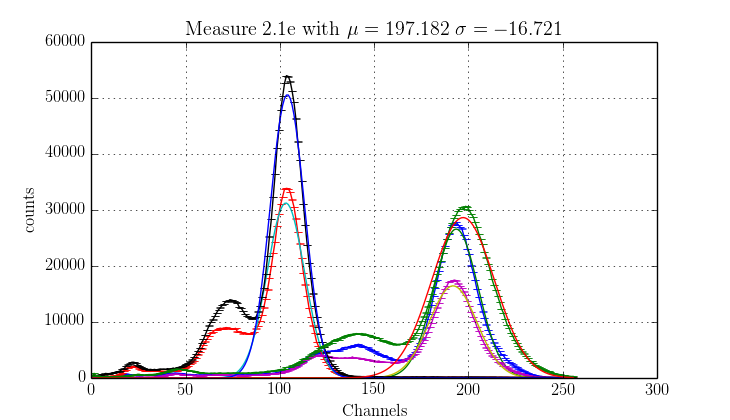
\includegraphics[width=\textwidth]{analysis/figures/plot2_1e}
        \caption{}
    \end{subfigure}
    \caption{Energy spectra with respect to the channels of the MCA, which we prescribed by
        measurements 2.1 (a) - (e).}
    \label{fig:sinus8}
\end{figure}
\begin{figure}[htpb]
    \centering
    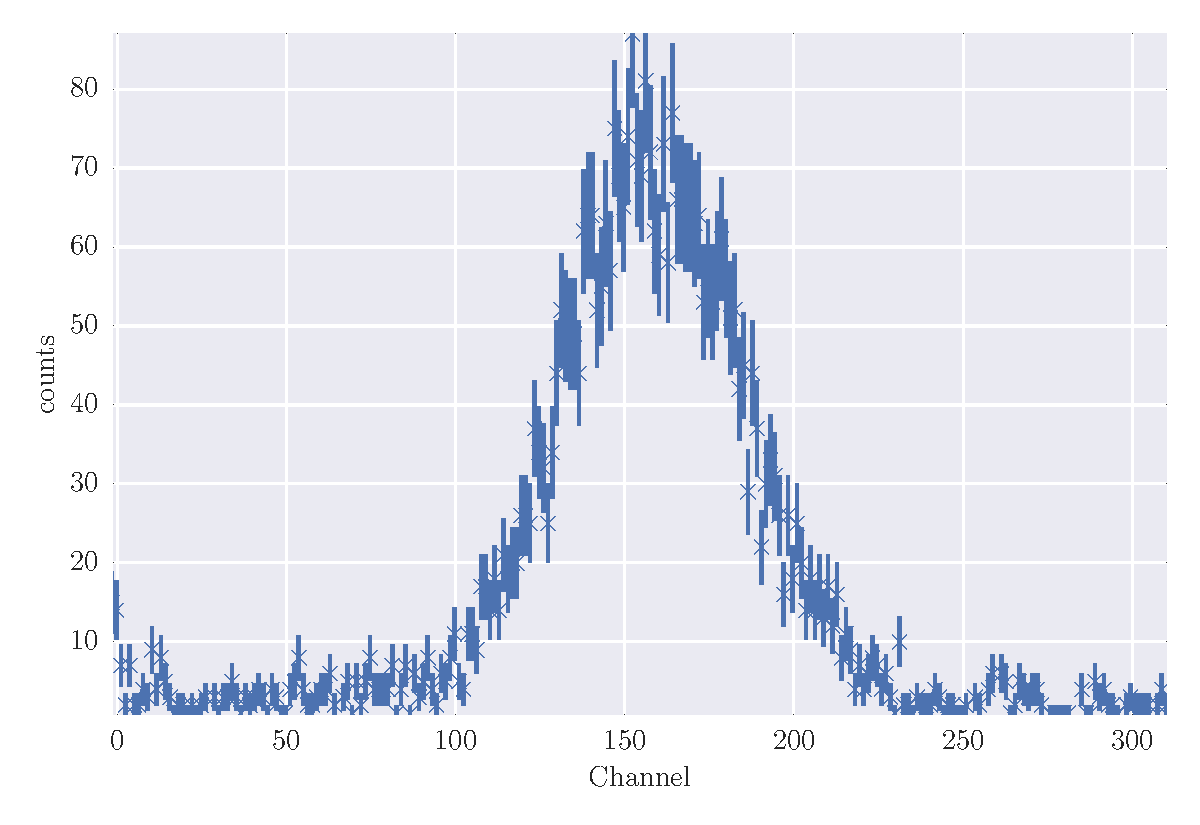
\includegraphics[width=1.0\linewidth]{analysis/figures/plot4_1}
    \caption{Measurement 4.1: $\Delta t $}
    \label{fig:4_1}
\end{figure}

\begin{figure}[htpb]
    \centering
    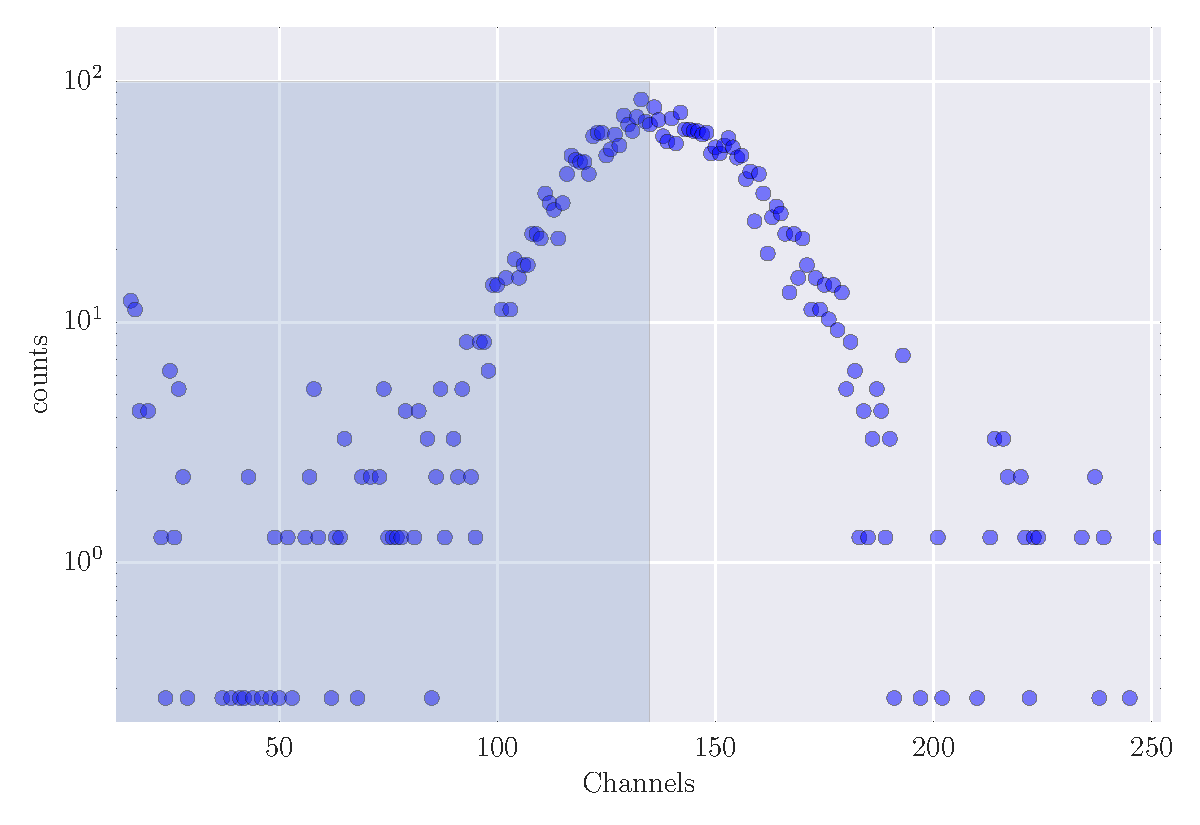
\includegraphics[width=1.0\linewidth]{analysis/figures/plot4_1_log}
    \caption{Measurement 4.1: $\Delta t $}
    \label{fig:4_1log}
\end{figure}


\begin{figure}[htpb]
    \centering
    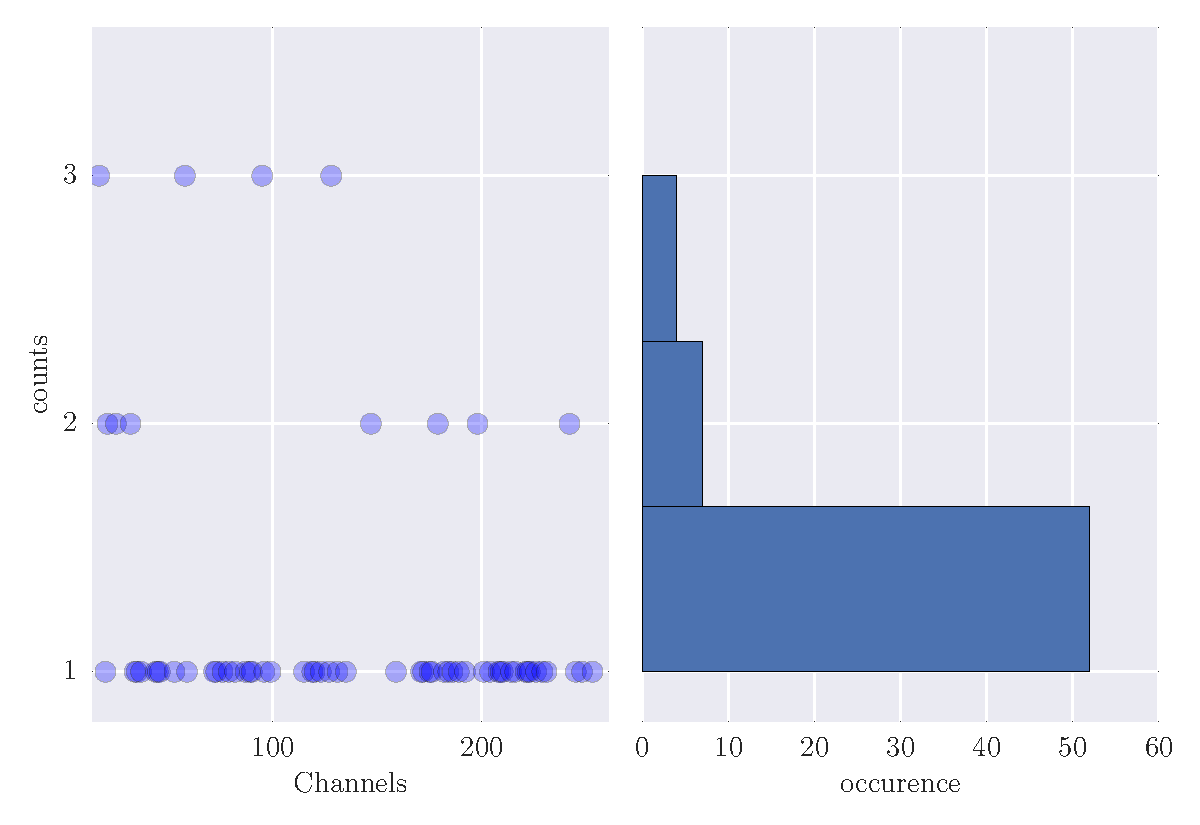
\includegraphics[width=1.0\linewidth]{analysis/figures/plot5_1_hist}
    \caption{Measurement 5.1: Random coincidences and their histogram.}
    \label{fig:5_1}
\end{figure}

